\section{Code Base}
This section outlines all the work done to produce the code, the design implementation and what the code can produce. 



\subsection{Set Up}
\subsubsection{Location}
All code can be found in the ./calpy/ directory, the code written for this research can be found in ./calpy/pause/ as well as extra plot code written in ./calpy/plots.

\subsubsection{Libraries Used}
\begin{itemize}
\item pydub.AudioSegment (WAV decoder) 
\item ffmpeg (requirement system install to use AudioSegment)
\item pandas (data handling)
\item numpy (data handling)
\item json (data handling)
\item matplotlib (plots)
\item seaborn (plots)
\item ptitprince (plots)
\item seaborn (plots)
\end{itemize}


\subsubsection{IDE}
Visual Studio Code was used to write everything due to its flexibility, lightweight and ease of use with running terminal commands.

 
\subsection{Design}
\subsubsection{Design goals}
The main goal was to make the code as sturdy, modularised and abstracted from the pause implementation as much as possible. It was also designed to be as readable and easily useable by others as possible. The main goals being:
\begin{itemize}
	\item Usability
	\item Replicability (for results)
	\item Error free (no bugs)
	\item System invariant (should work on windows and unix)
	\item Implementation invariance (i.e. if other prosodic speech elements are incorporated in the future, it should be trivial to incorporate)
\end{itemize}

Calpy already had a number of packages to use (e.g. DSP, plots, rqa, etc..). A pause package was created that sat on top of these functions, this included:
\paragraph{audio\_file\_.py:} All work required to digitise, symbolise, perform entropy and produce plots are done through the AudioFile class
\paragraph{data\_handling.py:} Data manipulation and formatting
\paragraph{dataset\_functions.py:} Collections of audio\_files were processed here
\paragraph{file\_handling.py:} Reading and writing to disk
\paragraph{parameters.py:} All initial input parameters for pause digitisation, symbol models, fast entropy settings and plot settings 
\paragraph{dataset\_folder.py:} Stored arrays of all the directories, files, frequencies and audio augmentations used \\

Modularising the code in this way made it more easily updatable, readable, design invariant and less prone to bugs. In total the pause package is roughly 1200-1300 lines of code. All audio files belong to an audio\_file\_ object that contains all the variables used and allows for meta-analysis on groups of audio\_file\_ objects all at once (e.g. histograms showing the difference in pauses amongst all the pause files). This minimised a lot of redundant work as the code generally had to be run over and over to ensure results were correct. All Audio files can be run by simply calling the directory, files and frequency from pre-defined arrays. An example of the main code can be seen in Figure 5.1: 
\begin{figure}[h]
	\begin{center}
		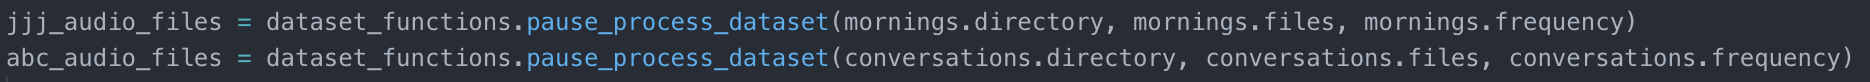
\includegraphics[scale=0.5]{src/main-matter/methodology/code-base/code/main}
		\caption{The code required in main to analyse all JJJ and ABC podcasts. This was designed to be as simple to compute as possible}
		\label{default}
	\end{center}
\end{figure}

These two lines create a collection of audio\_file\_ objects that can be used collectively. An example dataset can be seen in Figure 5.2.\\
\begin{figure}[h]
	\begin{center}
		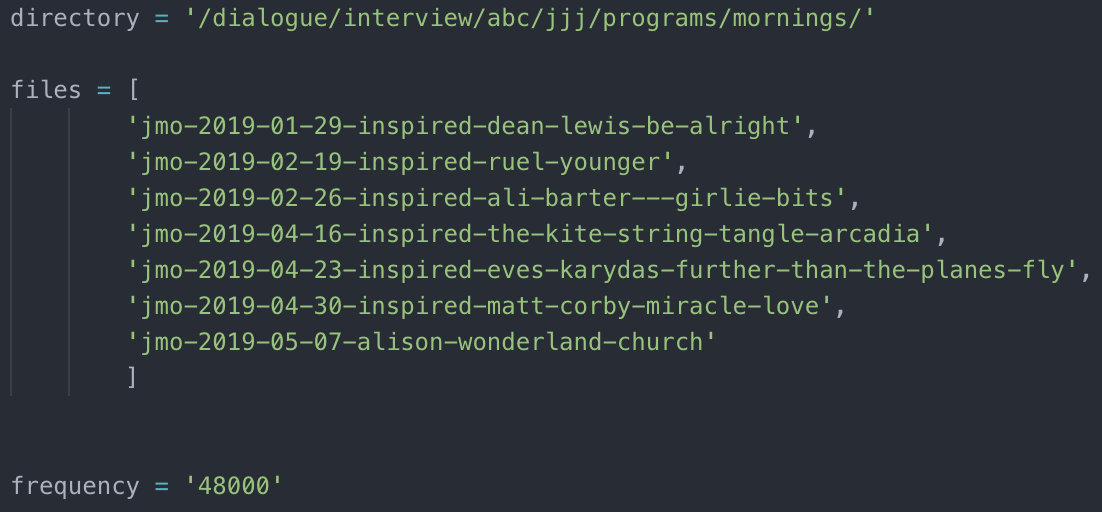
\includegraphics[scale=0.7]{src/main-matter/methodology/code-base/code/dataset}
		\caption{JJJ Mornings Dataset showing a list of files in a specified directory and their corresponding frequency}
		\label{default}
	\end{center}
\end{figure}
Test datasets were also made to ensure calpy is working and for finding bugs. These files are significantly lower in size than the actual files used (which can take 10-20 minutes to digitise). \\

\subsubsection{AudioFile Class}
AudioFile is split into 4 main parts:

\begin{enumerate}
	\item Digitisation
	\item Symbolisation
	\item Entropy
	\item Plots
\end{enumerate}

In brief, an audio file specified in main is turned into an audio\_file\_ object, this object will digitise the audio, symbolise it, produce the entropy profile, plot everything needed and output all variables calculated to file automatically. Each section requires input parameters to customise the output (e.g. min\_silence, bin\_sizes, symbol\_model, etc...). An example of the parameters of a given run can be seen in Figure 5.3. Everything produced from these sections finishes by writing to files and then reading them back. This effectively makes a checkpoint in the code that can be picked up on from later. Examples of the output variables can be seen in Figure 5.4 and 5.10-14. Once audio is digitised every other action can be done almost immediately with the saved digitised binary pause output. 

%Although this is good practice, it was really only worth doing for the digitisation process as this is the most time demanding. 

\begin{figure}[htbp]
	\begin{center}
		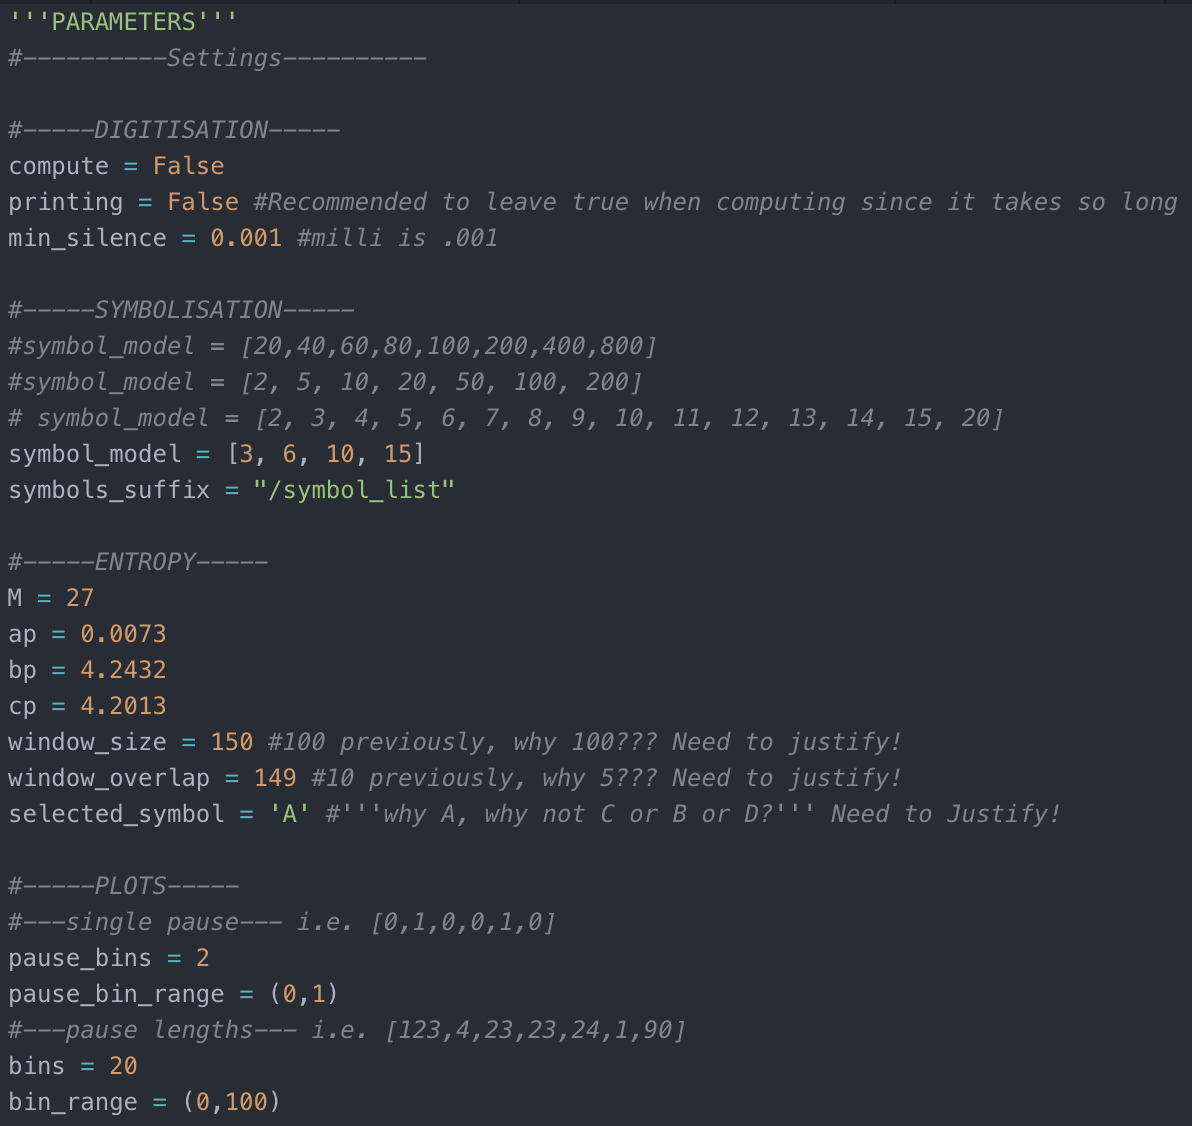
\includegraphics[scale=0.6]{src/main-matter/methodology/code-base/code/parameters}
		\caption{Example Parameter Setting for Calpy. These are required to run the analysis and control such parameters as the entropy window size, symbol model, and whether to recompute the digitised binary pause output}
		\label{default}
	\end{center}
\end{figure}

\subsubsection{Digitisation}
This turned audio files into 1's and 0's. The only parameter present for this section was min\_silence which recorded a pause for a given window of the audio file if a silence was present for as long as the min\_silence time given (e.g. a window of 100ms would be digitised as a pause if there existed a pause of length min\_silence (say 10ms) in that time frame). Min\_silence testing was done at 10ms, 1ms and .1ms and 1ms gave exponentially increasing time costs as the min\_silence value got shorter. \\
%but provided reasonable amounts of data back in terms of binary representations for each. 

Pauses of unbroken length (min of 1ms length used) were looked for and grouped as a single pause, the length of the pause being determined by the number of individual binary pauses that make up that pause. An example of the binary pause output can be seen in Figure 5.4 where a single pause is represented by an unbroken run of 0's, so the first pause from that file would be 2000ms because there is a run of 20 0's at the start of the output. Similarly for utterances where they are represented by 1's. %What about pauses that are unbroken by speech but broken by background sound? Maybe I should say that although we are looking for long pauses, its worth noting that finding long pauses is affected by the quality of the pause isolation. As the pause length goes on its more likely something will break it that incorrectly should not do so. \\

\begin{figure}[htbp]
	\begin{center}
		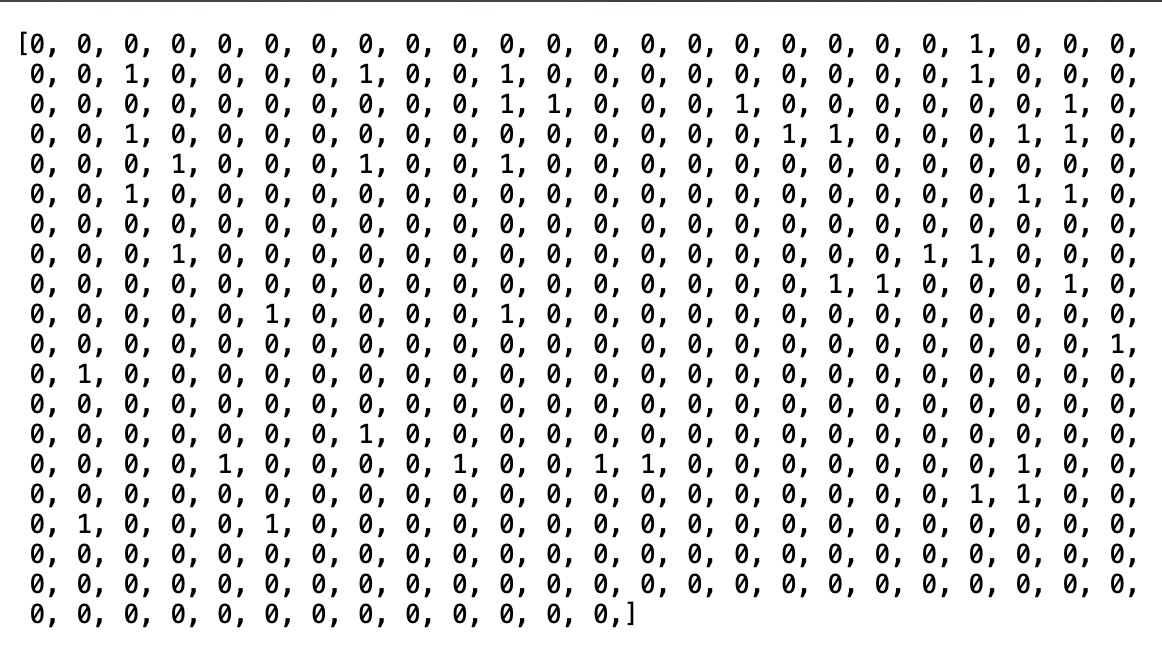
\includegraphics[scale=0.6]{src/main-matter/methodology/code-base/output/binary_pause}
		\caption{Example Binary Pause Output, where a single pause is represented by an unbroken run of 0's. The first pause from this file would be 2000ms because there is a run of 20 0's at the start of the output.}
		\label{default}
	\end{center}
\end{figure}


\subsubsection{Symbolisation}
Symbolisation was written to handle arbitrary symbol models as input without needing to change underlying implementation, meaning any bin size with any number of symbols can be created and modelled immediately (more precisely, the symbol model can be as long as the set of ascii characters). Capital letters are only used for readability purposes but the underlying code is able to use capital and lower case letters, numbers, special characters or any other ascii character as symbols. \\

Theoretically this allows for many types of pauses to be characterised (e.g. joint pause from speaker A to B, or vice versa, or inner pause of speaker A or inner pause of speaker B), however this isn't recommended until much more experiments is done and a much larger database of audio files can be drawn from to increase sample size. The symbolisation then automatically ranks the symbols based on the most frequently occurring to the least. When the symbols are ranked it can often be the case that they will not appear in alphabetic order, showing some pauses to be more frequent that are farther out. As shown in Figure 5.5 where B is the most frequently occurring and A is the least frequently occurring. \\
%Although literature from [paper] posits that there are 64 different types of pauses, it may hinder results to look for each distinct pause as very few samples will be able to be collected for each pause. This was deemed a potential future addition if enough data was found. \\

%While this code can be implemented to look for 64 distinct pauses and symbolise them accordingly, the data might not be sufficient to pull out data like that. 


\begin{figure}[htbp]
	\begin{center}
		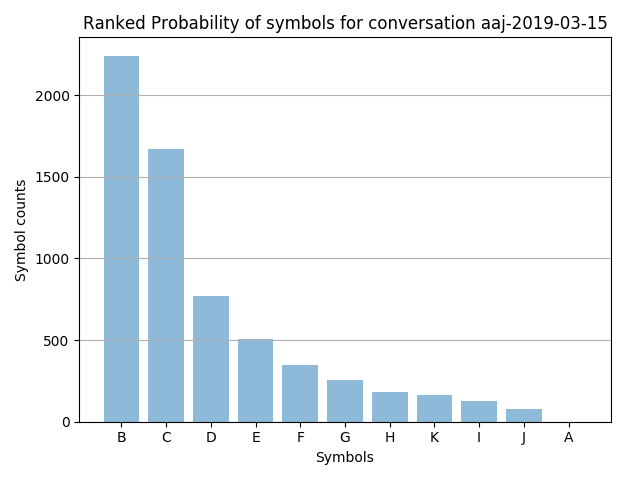
\includegraphics[scale=0.7]{src/main-matter/methodology/code-base/output/ranked_probability}
		\caption{Example Ranked Probability Plot where symbols are ordered by their likelihood of occurrence in the dataset. In this dataset B is the most frequently occurring and A is the least frequently occurring.}
		\label{default}
	\end{center}
\end{figure}

\subsubsection{Entropy} 
The novel Entropy method as outlined in [back] was initially incorporated into Calpy to reduce the computation time needed to produce entropy values. However, initial tests were on files with far greater symbol set sizes than what ended up existing for the audio files, meaning entropy calculations ended up being negligible in terms of time spent. This meant there was no noticeable difference in computation time between classic entropy and the novel entropy in terms of testing. Further tests were done using classic entropy as less parameters were required to be experimented with but the novel entropy was still written for the system. Accuracy change was negligible. 

\subsubsection{Plots}
In order to visualise the data and draw insight various plots were written that included histograms and raincloud plots to visualise pause distributions, utterance vs silence plots to showing the proportion of time spent pausing in an audio file, dual symbol probability ranking plots to show how one symbol set compares to another using the same symbol model, and anomaly plots to show how the entropy values change over time.

\begin{figure}[h!]
	\center
	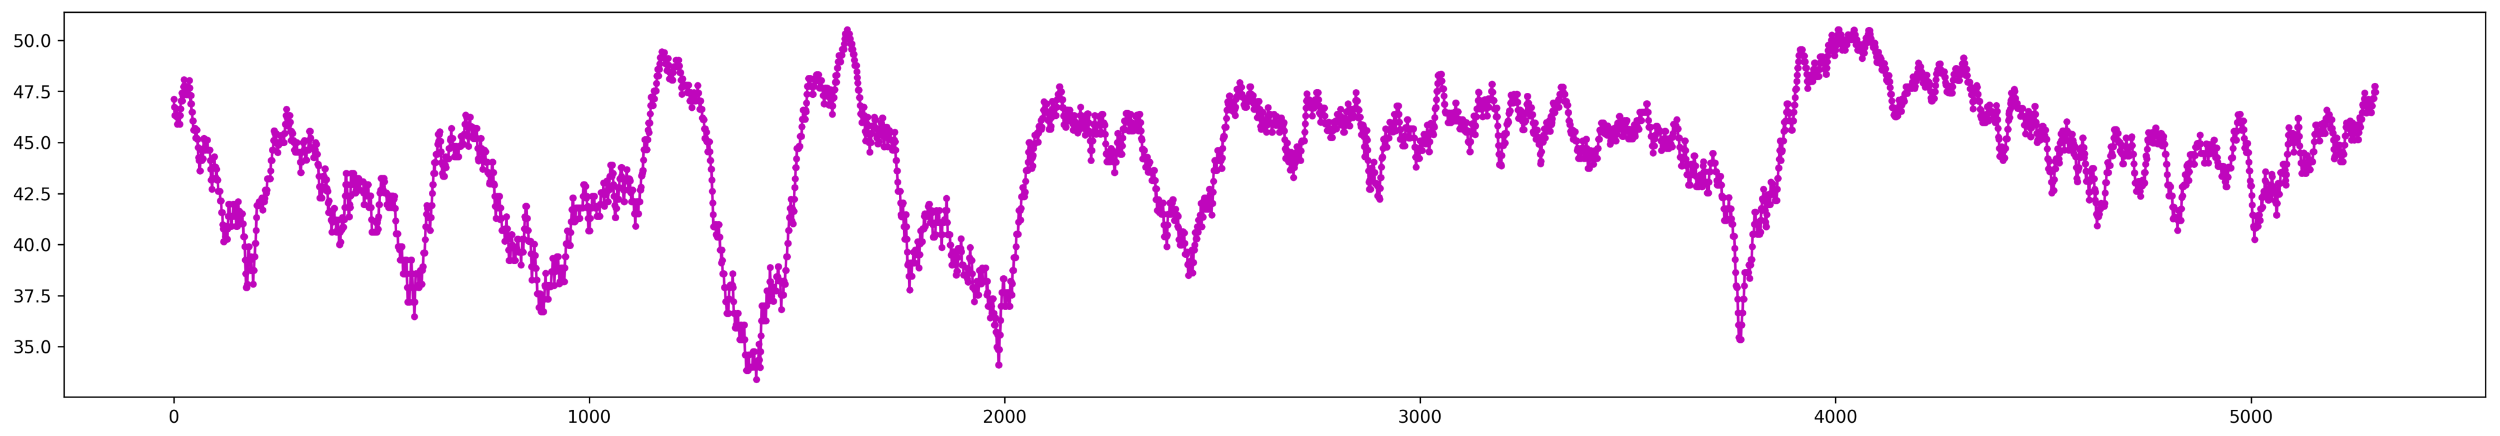
\includegraphics[scale=0.4]{src/main-matter/methodology/code-base/output/output_anomaly}
	\caption{Example Anomaly Plot shows the change in entropy over time for a given audio file. This is used to quickly visualise key properties of the entropy profile.}
	\label{fig:processing}
\end{figure}

\begin{figure}[h!]
	\center
	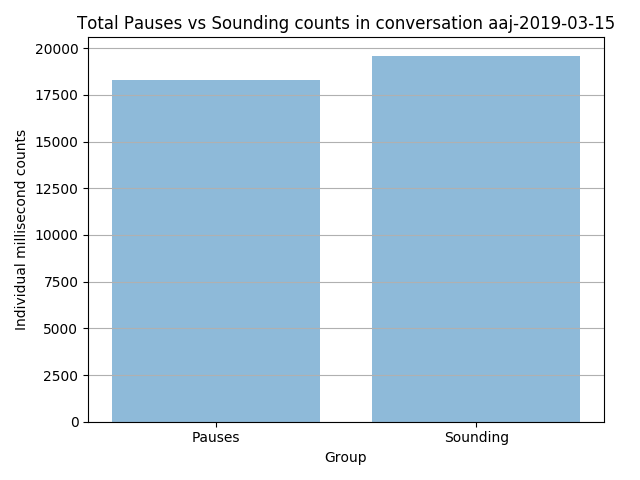
\includegraphics[scale=0.6]{src/main-matter/methodology/code-base/output/binary_pause_bar_chart}
	\caption{Example Sounding Plot shows the proportion of utterance to silence. This example shows an audio file with approximately 55\% of the file being utterances.}
	\label{fig:processing}
\end{figure}

\begin{figure}[h!]
	\center
	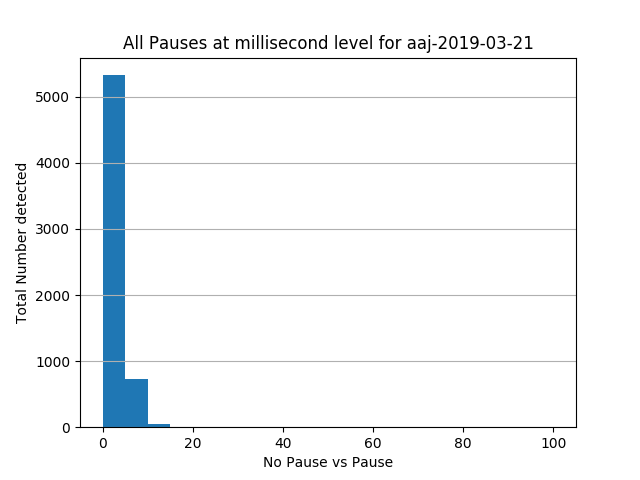
\includegraphics[scale=0.6]{src/main-matter/methodology/code-base/output/pause_histogram}
	\caption{Example Histogram Plot shows the distribution of pause lengths for a given audio file. This example shows a high proportion of audio files clustered around 1000ms.}
	\label{fig:processing}
\end{figure}

%\begin{figure}[h]
%	\center
%	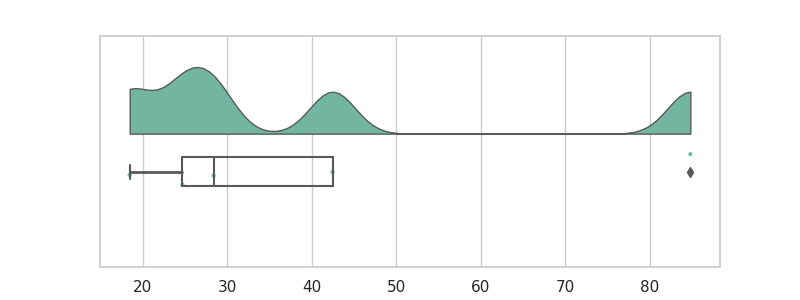
\includegraphics[scale=0.3]{src/main-matter/methodology/code-base/output/raincloud}
%	\caption{Example Anomaly Plot}
%	\label{fig:processing}
%\end{figure}

\begin{figure}[h!]
	\begin{center}
		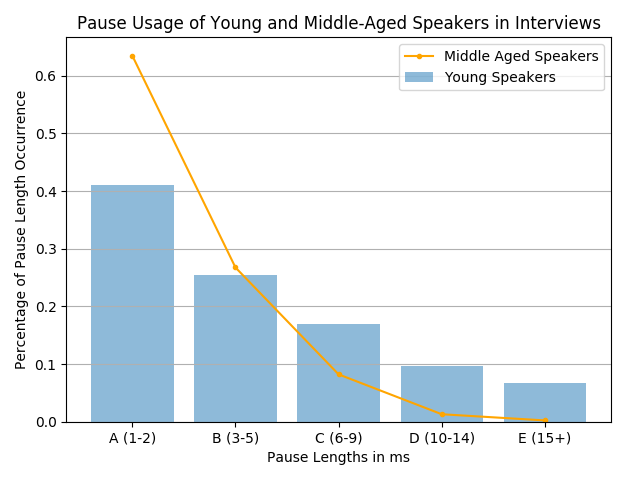
\includegraphics[scale=0.6]{src/main-matter/methodology/code-base/output/dual_ranked_probability}
		\caption{Example Ranked Probability Plot for a symbol model of [3, 6, 10, 15] where two datasets are shown, one in yellow and one in blue. This is useful to see how symbol models perform on audio files of separate groups.}
		\label{default}
	\end{center}
\end{figure}

\subsection{Required Input} All thats required are wav files of correct formatting and their file path. A range of frequencies are usable. Specifically 8000hz, 11025hz, 16000hz, 22050hz, 32000hz, 44100hz, 48000hz, 88200hz, 96000hz were all tested and accepted.

\subsection{Output} Upon completion all relevant output is automatically saved into a file structure dictated by the input folder structure (except now located in the output folder). Example: The file located at: 
\begin{verbatim}
'./data/interview/abc/jjj/programs/mornings/'
\end{verbatim}
would be output to 
\begin{verbatim}
'./output/interview/abc/jjj/programs/mornings/'.
\end{verbatim}

This was done to make file processing easier so only a file directory and a list of names was needed to process everything at once. 
It also allowed for easy reanalysis based upon work that had already been done without having to recompute previous work (which is costly). 
In order to streamline the process of gathering results, all variables generated throughout the procedure were sent to a text file (with some also being used in plots). Example text output files are shown below: \\

\begin{figure}[h!]
	\center
	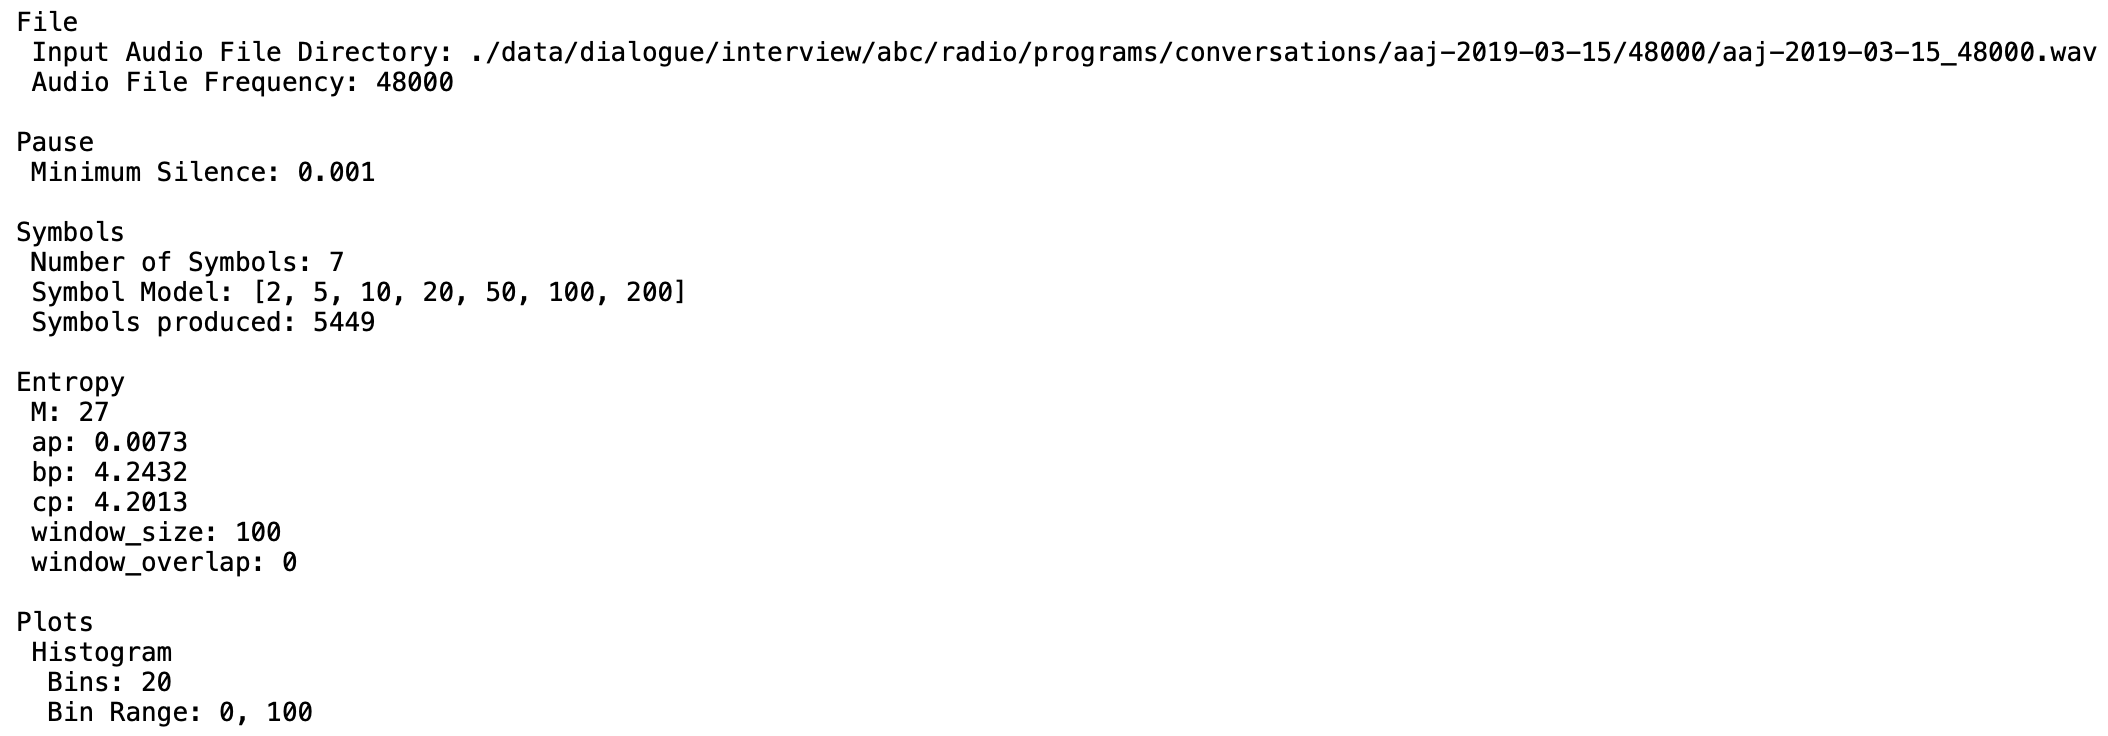
\includegraphics[scale=0.4]{src/main-matter/methodology/code-base/output/input_parameters}
	\caption{Example Code Parameters show what is recorded to disk after every program run. This ensures the correct input parameters can always be referred back to for any test or experiment that was performed.}
	\label{fig:parameters}
\end{figure}

\begin{figure}[h!]
	\center
	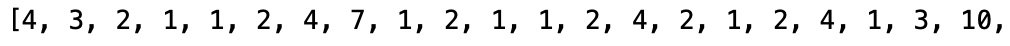
\includegraphics[scale=0.7]{src/main-matter/methodology/code-base/output/pauses}
	\caption{Example Pause Output shows what the pauses look like for an audio file. Each number represents a single pause of that length multiplied by 100ms. These values are derived from the binary pause output.}
	\label{fig:parameters}
\end{figure}

\begin{figure}[h!]
	\center
	
\includegraphics[scale=0.5]{src/main-matter/methodology/code-base/output/output_symbols}
	\caption{Example Output Symbols show what is required to perform entropy calculations. The symbol file will usually span 1000's of symbols.}
	\label{fig:processing}
\end{figure}

\begin{figure}[h!]
	\center
	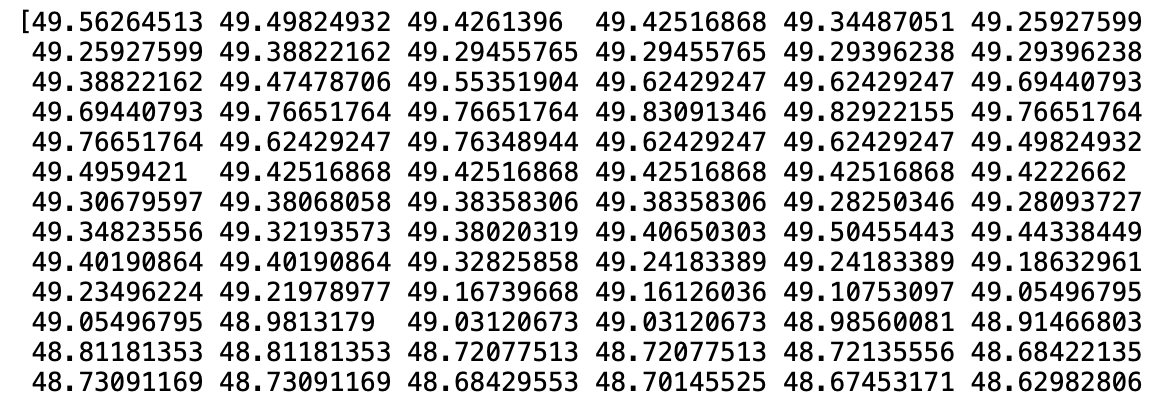
\includegraphics[scale=0.7]{src/main-matter/methodology/code-base/output/output_entropy}
	\caption{Example Output Entropy Profile shows what the entropy profile looks like. Generally the values for entropy are much lower, but specific values aren't important, its the relative change that matters.}
	\label{fig:processing}
\end{figure}

\begin{figure}[h!]
	\center
	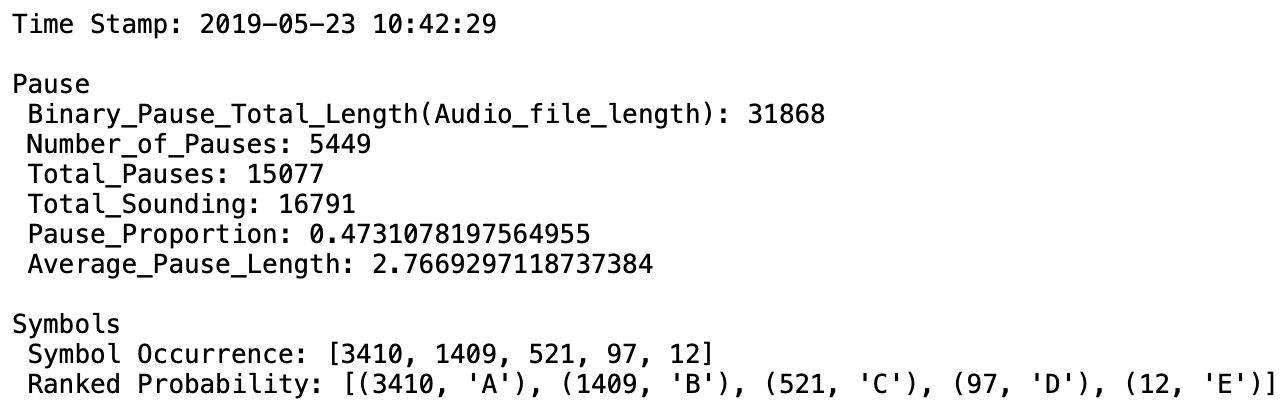
\includegraphics[scale=0.6]{src/main-matter/methodology/code-base/output/output_data}
	\caption{Example General Output Data shows general properties of the audio file and it's pauses. This is produced for every audio file analysed automatically.}
	\label{fig:processing}
\end{figure}


\newpage

